\documentclass[1p]{elsarticle_modified}
%\bibliographystyle{elsarticle-num}

%\usepackage[colorlinks]{hyperref}
%\usepackage{abbrmath_seonhwa} %\Abb, \Ascr, \Acal ,\Abf, \Afrak
\usepackage{amsfonts}
\usepackage{amssymb}
\usepackage{amsmath}
\usepackage{amsthm}
\usepackage{scalefnt}
\usepackage{amsbsy}
\usepackage{kotex}
\usepackage{caption}
\usepackage{subfig}
\usepackage{color}
\usepackage{graphicx}
\usepackage{xcolor} %% white, black, red, green, blue, cyan, magenta, yellow
\usepackage{float}
\usepackage{setspace}
\usepackage{hyperref}

\usepackage{tikz}
\usetikzlibrary{arrows}

\usepackage{multirow}
\usepackage{array} % fixed length table
\usepackage{hhline}

%%%%%%%%%%%%%%%%%%%%%
\makeatletter
\renewcommand*\env@matrix[1][\arraystretch]{%
	\edef\arraystretch{#1}%
	\hskip -\arraycolsep
	\let\@ifnextchar\new@ifnextchar
	\array{*\c@MaxMatrixCols c}}
\makeatother %https://tex.stackexchange.com/questions/14071/how-can-i-increase-the-line-spacing-in-a-matrix
%%%%%%%%%%%%%%%

\usepackage[normalem]{ulem}

\newcommand{\msout}[1]{\ifmmode\text{\sout{\ensuremath{#1}}}\else\sout{#1}\fi}
%SOURCE: \msout is \stkout macro in https://tex.stackexchange.com/questions/20609/strikeout-in-math-mode

\newcommand{\cancel}[1]{
	\ifmmode
	{\color{red}\msout{#1}}
	\else
	{\color{red}\sout{#1}}
	\fi
}

\newcommand{\add}[1]{
	{\color{blue}\uwave{#1}}
}

\newcommand{\replace}[2]{
	\ifmmode
	{\color{red}\msout{#1}}{\color{blue}\uwave{#2}}
	\else
	{\color{red}\sout{#1}}{\color{blue}\uwave{#2}}
	\fi
}

\newcommand{\Sol}{\mathcal{S}} %segment
\newcommand{\D}{D} %diagram
\newcommand{\A}{\mathcal{A}} %arc


%%%%%%%%%%%%%%%%%%%%%%%%%%%%%5 test

\def\sl{\operatorname{\textup{SL}}(2,\Cbb)}
\def\psl{\operatorname{\textup{PSL}}(2,\Cbb)}
\def\quan{\mkern 1mu \triangleright \mkern 1mu}

\theoremstyle{definition}
\newtheorem{thm}{Theorem}[section]
\newtheorem{prop}[thm]{Proposition}
\newtheorem{lem}[thm]{Lemma}
\newtheorem{ques}[thm]{Question}
\newtheorem{cor}[thm]{Corollary}
\newtheorem{defn}[thm]{Definition}
\newtheorem{exam}[thm]{Example}
\newtheorem{rmk}[thm]{Remark}
\newtheorem{alg}[thm]{Algorithm}

\newcommand{\I}{\sqrt{-1}}
\begin{document}

%\begin{frontmatter}
%
%\title{Boundary parabolic representations of knots up to 8 crossings}
%
%%% Group authors per affiliation:
%\author{Yunhi Cho} 
%\address{Department of Mathematics, University of Seoul, Seoul, Korea}
%\ead{yhcho@uos.ac.kr}
%
%
%\author{Seonhwa Kim} %\fnref{s_kim}}
%\address{Center for Geometry and Physics, Institute for Basic Science, Pohang, 37673, Korea}
%\ead{ryeona17@ibs.re.kr}
%
%\author{Hyuk Kim}
%\address{Department of Mathematical Sciences, Seoul National University, Seoul 08826, Korea}
%\ead{hyukkim@snu.ac.kr}
%
%\author{Seokbeom Yoon}
%\address{Department of Mathematical Sciences, Seoul National University, Seoul, 08826,  Korea}
%\ead{sbyoon15@snu.ac.kr}
%
%\begin{abstract}
%We find all boundary parabolic representation of knots up to 8 crossings.
%
%\end{abstract}
%\begin{keyword}
%    \MSC[2010] 57M25 
%\end{keyword}
%
%\end{frontmatter}

%\linenumbers
%\tableofcontents
%
\newcommand\colored[1]{\textcolor{white}{\rule[-0.35ex]{0.8em}{1.4ex}}\kern-0.8em\color{red} #1}%
%\newcommand\colored[1]{\textcolor{white}{ #1}\kern-2.17ex	\textcolor{white}{ #1}\kern-1.81ex	\textcolor{white}{ #1}\kern-2.15ex\color{red}#1	}

{\Large $\underline{12n_{0370}~(K12n_{0370})}$}

\setlength{\tabcolsep}{10pt}
\renewcommand{\arraystretch}{1.6}
\vspace{1cm}\begin{tabular}{m{100pt}>{\centering\arraybackslash}m{274pt}}
\multirow{5}{120pt}{
	\centering
	\includegraphics[width=112pt]{../../../GIT/diagram.site/Diagrams/png/2459_12n_0370.png}\\
\ \ \ A knot diagram\footnotemark}&
\allowdisplaybreaks
\textbf{Linearized knot diagam} \\
\cline{2-2}
 &
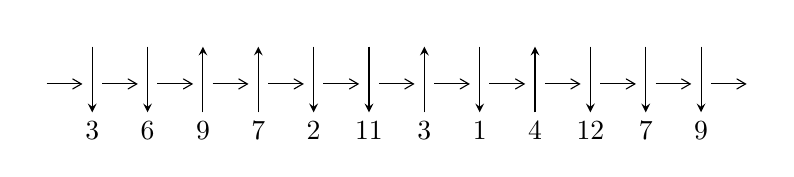
\begin{tikzpicture}[x=20pt, y=17pt]
	% nodes
	\node (C0) at (0, 0) {};
	\node (C1) at (1, 0) {};
	\node (C1U) at (1, +1) {};
	\node (C1D) at (1, -1) {3};

	\node (C2) at (2, 0) {};
	\node (C2U) at (2, +1) {};
	\node (C2D) at (2, -1) {6};

	\node (C3) at (3, 0) {};
	\node (C3U) at (3, +1) {};
	\node (C3D) at (3, -1) {9};

	\node (C4) at (4, 0) {};
	\node (C4U) at (4, +1) {};
	\node (C4D) at (4, -1) {7};

	\node (C5) at (5, 0) {};
	\node (C5U) at (5, +1) {};
	\node (C5D) at (5, -1) {2};

	\node (C6) at (6, 0) {};
	\node (C6U) at (6, +1) {};
	\node (C6D) at (6, -1) {11};

	\node (C7) at (7, 0) {};
	\node (C7U) at (7, +1) {};
	\node (C7D) at (7, -1) {3};

	\node (C8) at (8, 0) {};
	\node (C8U) at (8, +1) {};
	\node (C8D) at (8, -1) {1};

	\node (C9) at (9, 0) {};
	\node (C9U) at (9, +1) {};
	\node (C9D) at (9, -1) {4};

	\node (C10) at (10, 0) {};
	\node (C10U) at (10, +1) {};
	\node (C10D) at (10, -1) {12};

	\node (C11) at (11, 0) {};
	\node (C11U) at (11, +1) {};
	\node (C11D) at (11, -1) {7};

	\node (C12) at (12, 0) {};
	\node (C12U) at (12, +1) {};
	\node (C12D) at (12, -1) {9};
	\node (C13) at (13, 0) {};

	% arrows
	\draw[->,>={angle 60}]
	(C0) edge (C1) (C1) edge (C2) (C2) edge (C3) (C3) edge (C4) (C4) edge (C5) (C5) edge (C6) (C6) edge (C7) (C7) edge (C8) (C8) edge (C9) (C9) edge (C10) (C10) edge (C11) (C11) edge (C12) (C12) edge (C13) ;	\draw[->,>=stealth]
	(C1U) edge (C1D) (C2U) edge (C2D) (C3D) edge (C3U) (C4D) edge (C4U) (C5U) edge (C5D) (C6U) edge (C6D) (C7D) edge (C7U) (C8U) edge (C8D) (C9D) edge (C9U) (C10U) edge (C10D) (C11U) edge (C11D) (C12U) edge (C12D) ;
	\end{tikzpicture} \\
\hhline{~~} \\& 
\textbf{Solving Sequence} \\ \cline{2-2} 
 &
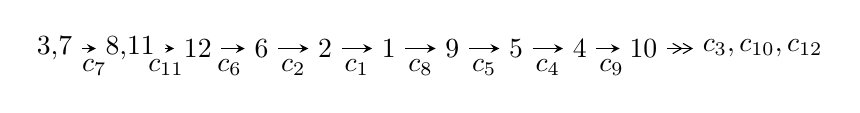
\begin{tikzpicture}[x=23pt, y=7pt]
	% node
	\node (A0) at (-1/8, 0) {3,7};
	\node (A1) at (17/16, 0) {8,11};
	\node (A2) at (17/8, 0) {12};
	\node (A3) at (25/8, 0) {6};
	\node (A4) at (33/8, 0) {2};
	\node (A5) at (41/8, 0) {1};
	\node (A6) at (49/8, 0) {9};
	\node (A7) at (57/8, 0) {5};
	\node (A8) at (65/8, 0) {4};
	\node (A9) at (73/8, 0) {10};
	\node (C1) at (1/2, -1) {$c_{7}$};
	\node (C2) at (13/8, -1) {$c_{11}$};
	\node (C3) at (21/8, -1) {$c_{6}$};
	\node (C4) at (29/8, -1) {$c_{2}$};
	\node (C5) at (37/8, -1) {$c_{1}$};
	\node (C6) at (45/8, -1) {$c_{8}$};
	\node (C7) at (53/8, -1) {$c_{5}$};
	\node (C8) at (61/8, -1) {$c_{4}$};
	\node (C9) at (69/8, -1) {$c_{9}$};
	\node (A10) at (11, 0) {$c_{3},c_{10},c_{12}$};

	% edge
	\draw[->,>=stealth]	
	(A0) edge (A1) (A1) edge (A2) (A2) edge (A3) (A3) edge (A4) (A4) edge (A5) (A5) edge (A6) (A6) edge (A7) (A7) edge (A8) (A8) edge (A9) ;
	\draw[->>,>={angle 60}]	
	(A9) edge (A10);
\end{tikzpicture} \\ 

\end{tabular} \\

\footnotetext{
The image of knot diagram is generated by the software ``\textbf{Draw programme}" developed by Andrew Bartholomew(\url{http://www.layer8.co.uk/maths/draw/index.htm\#Running-draw}), where we modified some parts for our purpose(\url{https://github.com/CATsTAILs/LinksPainter}).
}\phantom \\ \newline 
\centering \textbf{Ideals for irreducible components\footnotemark of $X_{\text{par}}$} 
 
\begin{align*}
I^u_{1}&=\langle 
1.28847\times10^{15} u^{11}-4.74420\times10^{14} u^{10}+\cdots+8.72123\times10^{16} b+2.22344\times10^{17},\\
\phantom{I^u_{1}}&\phantom{= \langle  }1.00938\times10^{15} u^{11}-1.97502\times10^{14} u^{10}+\cdots+8.72123\times10^{16} a+3.30952\times10^{17},\\
\phantom{I^u_{1}}&\phantom{= \langle  }u^{12}-34 u^{10}-10 u^9+374 u^8+256 u^7-1158 u^6-838 u^5+1243 u^4+1159 u^3+685 u^2+342 u+61\rangle \\
I^u_{2}&=\langle 
-491 u^9-169 u^8+138 u^7+2797 u^6-952 u^5-2978 u^4-1762 u^3+4940 u^2+1423 b+1946 u-997,\\
\phantom{I^u_{2}}&\phantom{= \langle  }120 u^9+363 u^8-709 u^7-501 u^6-1399 u^5+5504 u^4-1259 u^3-2839 u^2+1423 a-3481 u+4617,\\
\phantom{I^u_{2}}&\phantom{= \langle  }u^{10}- u^9-5 u^7+9 u^6-3 u^4-9 u^3+9 u^2- u-1\rangle \\
\\
\end{align*}
\raggedright * 2 irreducible components of $\dim_{\mathbb{C}}=0$, with total 22 representations.\\
\footnotetext{All coefficients of polynomials are rational numbers. But the coefficients are sometimes approximated in decimal forms when there is not enough margin.}
\newpage
\renewcommand{\arraystretch}{1}
\centering \section*{I. $I^u_{1}= \langle 1.29\times10^{15} u^{11}-4.74\times10^{14} u^{10}+\cdots+8.72\times10^{16} b+2.22\times10^{17},\;1.01\times10^{15} u^{11}-1.98\times10^{14} u^{10}+\cdots+8.72\times10^{16} a+3.31\times10^{17},\;u^{12}-34 u^{10}+\cdots+342 u+61 \rangle$}
\flushleft \textbf{(i) Arc colorings}\\
\begin{tabular}{m{7pt} m{180pt} m{7pt} m{180pt} }
\flushright $a_{3}=$&$\begin{pmatrix}0\\u\end{pmatrix}$ \\
\flushright $a_{7}=$&$\begin{pmatrix}1\\0\end{pmatrix}$ \\
\flushright $a_{8}=$&$\begin{pmatrix}1\\- u^2\end{pmatrix}$ \\
\flushright $a_{11}=$&$\begin{pmatrix}-0.0115739 u^{11}+0.00226461 u^{10}+\cdots-3.98267 u-3.79478\\-0.0147739 u^{11}+0.00543983 u^{10}+\cdots-6.01362 u-2.54946\end{pmatrix}$ \\
\flushright $a_{12}=$&$\begin{pmatrix}0.00320005 u^{11}-0.00317522 u^{10}+\cdots+2.03095 u-1.24533\\-0.0147739 u^{11}+0.00543983 u^{10}+\cdots-6.01362 u-2.54946\end{pmatrix}$ \\
\flushright $a_{6}=$&$\begin{pmatrix}-0.0414649 u^{11}+0.0165212 u^{10}+\cdots-17.1890 u-6.03303\\-0.00596827 u^{11}+0.00228246 u^{10}+\cdots-2.07003 u-1.25196\end{pmatrix}$ \\
\flushright $a_{2}=$&$\begin{pmatrix}0.0163711 u^{11}-0.00810347 u^{10}+\cdots+7.17353 u+1.18110\\-0.00876668 u^{11}+0.00418598 u^{10}+\cdots-3.18088 u-1.53147\end{pmatrix}$ \\
\flushright $a_{1}=$&$\begin{pmatrix}0.0163711 u^{11}-0.00810347 u^{10}+\cdots+7.17353 u+1.18110\\-0.0125049 u^{11}+0.00522621 u^{10}+\cdots-4.95363 u-2.02578\end{pmatrix}$ \\
\flushright $a_{9}=$&$\begin{pmatrix}0.00757115 u^{11}-0.00279404 u^{10}+\cdots+2.94107 u+2.37499\\0.00556736 u^{11}-0.00252772 u^{10}+\cdots+2.05708 u+0.942635\end{pmatrix}$ \\
\flushright $a_{5}=$&$\begin{pmatrix}-0.00964076 u^{11}+0.00285039 u^{10}+\cdots-2.23827 u-1.62408\\-0.00279404 u^{11}+0.000870939 u^{10}+\cdots-0.214346 u-0.461840\end{pmatrix}$ \\
\flushright $a_{4}=$&$\begin{pmatrix}-0.00684672 u^{11}+0.00197945 u^{10}+\cdots-2.02393 u-1.16224\\-0.00279404 u^{11}+0.000870939 u^{10}+\cdots-0.214346 u-0.461840\end{pmatrix}$ \\
\flushright $a_{10}=$&$\begin{pmatrix}0.00416895 u^{11}-0.00269474 u^{10}+\cdots+0.812978 u+1.59345\\0.00358791 u^{11}-0.00224683 u^{10}+\cdots+0.877740 u+0.524985\end{pmatrix}$\\&\end{tabular}
\flushleft \textbf{(ii) Obstruction class $= -1$}\\~\\
\flushleft \textbf{(iii) Cusp Shapes $= -\frac{8580809856421526}{87212327051456087} u^{11}+\frac{3421020397474812}{87212327051456087} u^{10}+\cdots-\frac{4710390701175382035}{87212327051456087} u-\frac{26157625863371374}{1429710279532067}$}\\~\\
\newpage\renewcommand{\arraystretch}{1}
\flushleft \textbf{(iv) u-Polynomials at the component}\newline \\
\begin{tabular}{m{50pt}|m{274pt}}
Crossings & \hspace{64pt}u-Polynomials at each crossing \\
\hline $$\begin{aligned}c_{1}\end{aligned}$$&$\begin{aligned}
&u^{12}+10 u^{10}+\cdots+3 u+1
\end{aligned}$\\
\hline $$\begin{aligned}c_{2},c_{5}\end{aligned}$$&$\begin{aligned}
&u^{12}+4 u^{11}+\cdots- u-1
\end{aligned}$\\
\hline $$\begin{aligned}c_{3},c_{4},c_{9}\end{aligned}$$&$\begin{aligned}
&u^{12}+u^{11}+\cdots+4 u+1
\end{aligned}$\\
\hline $$\begin{aligned}c_{6},c_{11}\end{aligned}$$&$\begin{aligned}
&u^{12}-8 u^{11}+\cdots+10 u-4
\end{aligned}$\\
\hline $$\begin{aligned}c_{7}\end{aligned}$$&$\begin{aligned}
&u^{12}-34 u^{10}+\cdots+342 u+61
\end{aligned}$\\
\hline $$\begin{aligned}c_{8},c_{12}\end{aligned}$$&$\begin{aligned}
&u^{12}- u^{11}+\cdots+13 u-1
\end{aligned}$\\
\hline $$\begin{aligned}c_{10}\end{aligned}$$&$\begin{aligned}
&u^{12}+4 u^{11}+\cdots+44 u+16
\end{aligned}$\\
\hline
\end{tabular}\\~\\
\newpage\renewcommand{\arraystretch}{1}
\flushleft \textbf{(v) Riley Polynomials at the component}\newline \\
\begin{tabular}{m{50pt}|m{274pt}}
Crossings & \hspace{64pt}Riley Polynomials at each crossing \\
\hline $$\begin{aligned}c_{1}\end{aligned}$$&$\begin{aligned}
&y^{12}+20 y^{11}+\cdots-3 y+1
\end{aligned}$\\
\hline $$\begin{aligned}c_{2},c_{5}\end{aligned}$$&$\begin{aligned}
&y^{12}+10 y^{10}+\cdots-3 y+1
\end{aligned}$\\
\hline $$\begin{aligned}c_{3},c_{4},c_{9}\end{aligned}$$&$\begin{aligned}
&y^{12}-29 y^{11}+\cdots-12 y+1
\end{aligned}$\\
\hline $$\begin{aligned}c_{6},c_{11}\end{aligned}$$&$\begin{aligned}
&y^{12}-4 y^{11}+\cdots-44 y+16
\end{aligned}$\\
\hline $$\begin{aligned}c_{7}\end{aligned}$$&$\begin{aligned}
&y^{12}-68 y^{11}+\cdots-33394 y+3721
\end{aligned}$\\
\hline $$\begin{aligned}c_{8},c_{12}\end{aligned}$$&$\begin{aligned}
&y^{12}+33 y^{11}+\cdots-269 y+1
\end{aligned}$\\
\hline $$\begin{aligned}c_{10}\end{aligned}$$&$\begin{aligned}
&y^{12}+48 y^{11}+\cdots+3216 y+256
\end{aligned}$\\
\hline
\end{tabular}\\~\\
\newpage\flushleft \textbf{(vi) Complex Volumes and Cusp Shapes}
$$\begin{array}{c|c|c}  
\text{Solutions to }I^u_{1}& \I (\text{vol} + \sqrt{-1}CS) & \text{Cusp shape}\\
 \hline 
\begin{aligned}
u &= -0.015982 + 0.502004 I \\
a &= -1.33976 + 0.88379 I \\
b &= -0.373800 + 0.452174 I\end{aligned}
 & -0.313401 + 1.169960 I & -3.81973 - 5.53143 I \\ \hline\begin{aligned}
u &= -0.015982 - 0.502004 I \\
a &= -1.33976 - 0.88379 I \\
b &= -0.373800 - 0.452174 I\end{aligned}
 & -0.313401 - 1.169960 I & -3.81973 + 5.53143 I \\ \hline\begin{aligned}
u &= -0.487209\phantom{ +0.000000I} \\
a &= -1.96376\phantom{ +0.000000I} \\
b &= \phantom{-}0.690624\phantom{ +0.000000I}\end{aligned}
 & -2.57792\phantom{ +0.000000I} & \phantom{-}8.93780\phantom{ +0.000000I} \\ \hline\begin{aligned}
u &= \phantom{-}1.53808 + 0.50690 I \\
a &= \phantom{-}0.700750 + 0.138104 I \\
b &= \phantom{-}0.742800 - 0.761818 I\end{aligned}
 & \phantom{-}3.43038 + 0.92181 I & \phantom{-}0.166703 - 0.576827 I \\ \hline\begin{aligned}
u &= \phantom{-}1.53808 - 0.50690 I \\
a &= \phantom{-}0.700750 - 0.138104 I \\
b &= \phantom{-}0.742800 + 0.761818 I\end{aligned}
 & \phantom{-}3.43038 - 0.92181 I & \phantom{-}0.166703 + 0.576827 I \\ \hline\begin{aligned}
u &= -1.64293 + 0.28456 I \\
a &= \phantom{-}1.107820 - 0.267147 I \\
b &= \phantom{-}0.969113 + 0.706030 I\end{aligned}
 & \phantom{-}2.73449 - 4.65154 I & -0.40649 + 6.35112 I \\ \hline\begin{aligned}
u &= -1.64293 - 0.28456 I \\
a &= \phantom{-}1.107820 + 0.267147 I \\
b &= \phantom{-}0.969113 - 0.706030 I\end{aligned}
 & \phantom{-}2.73449 + 4.65154 I & -0.40649 - 6.35112 I \\ \hline\begin{aligned}
u &= -0.299850\phantom{ +0.000000I} \\
a &= -2.90979\phantom{ +0.000000I} \\
b &= -0.917503\phantom{ +0.000000I}\end{aligned}
 & -1.69975\phantom{ +0.000000I} & -3.47970\phantom{ +0.000000I} \\ \hline\begin{aligned}
u &= -3.60163 + 0.13896 I \\
a &= \phantom{-}0.400586 + 0.118619 I \\
b &= \phantom{-}1.42147 - 1.15303 I\end{aligned}
 & -12.68910 + 1.00394 I & -1.189954 + 0.108309 I \\ \hline\begin{aligned}
u &= -3.60163 - 0.13896 I \\
a &= \phantom{-}0.400586 - 0.118619 I \\
b &= \phantom{-}1.42147 + 1.15303 I\end{aligned}
 & -12.68910 - 1.00394 I & -1.189954 - 0.108309 I\\
 \hline 
 \end{array}$$\newpage$$\begin{array}{c|c|c}  
\text{Solutions to }I^u_{1}& \I (\text{vol} + \sqrt{-1}CS) & \text{Cusp shape}\\
 \hline 
\begin{aligned}
u &= \phantom{-}4.11599 + 0.72988 I \\
a &= \phantom{-}0.591968 + 0.319795 I \\
b &= \phantom{-}1.35386 - 1.23724 I\end{aligned}
 & -12.4077 + 8.7999 I & -0.97957 - 3.65752 I \\ \hline\begin{aligned}
u &= \phantom{-}4.11599 - 0.72988 I \\
a &= \phantom{-}0.591968 - 0.319795 I \\
b &= \phantom{-}1.35386 + 1.23724 I\end{aligned}
 & -12.4077 - 8.7999 I & -0.97957 + 3.65752 I\\
 \hline 
 \end{array}$$\newpage\newpage\renewcommand{\arraystretch}{1}
\centering \section*{II. $I^u_{2}= \langle -491 u^9-169 u^8+\cdots+1423 b-997,\;120 u^9+363 u^8+\cdots+1423 a+4617,\;u^{10}- u^9-5 u^7+9 u^6-3 u^4-9 u^3+9 u^2- u-1 \rangle$}
\flushleft \textbf{(i) Arc colorings}\\
\begin{tabular}{m{7pt} m{180pt} m{7pt} m{180pt} }
\flushright $a_{3}=$&$\begin{pmatrix}0\\u\end{pmatrix}$ \\
\flushright $a_{7}=$&$\begin{pmatrix}1\\0\end{pmatrix}$ \\
\flushright $a_{8}=$&$\begin{pmatrix}1\\- u^2\end{pmatrix}$ \\
\flushright $a_{11}=$&$\begin{pmatrix}-0.0843289 u^{9}-0.255095 u^{8}+\cdots+2.44624 u-3.24455\\0.345046 u^{9}+0.118763 u^{8}+\cdots-1.36753 u+0.700632\end{pmatrix}$ \\
\flushright $a_{12}=$&$\begin{pmatrix}-0.429375 u^{9}-0.373858 u^{8}+\cdots+3.81377 u-3.94519\\0.345046 u^{9}+0.118763 u^{8}+\cdots-1.36753 u+0.700632\end{pmatrix}$ \\
\flushright $a_{6}=$&$\begin{pmatrix}-0.454673 u^{9}+0.849613 u^{8}+\cdots-7.55235 u+1.78145\\1.04287 u^{9}-0.545327 u^{8}+\cdots+3.31483 u+0.824315\end{pmatrix}$ \\
\flushright $a_{2}=$&$\begin{pmatrix}0.613493 u^{9}-0.919185 u^{8}+\cdots+7.12860 u-2.12087\\-0.781448 u^{9}+0.236121 u^{8}+\cdots-2.19817 u-0.666198\end{pmatrix}$ \\
\flushright $a_{1}=$&$\begin{pmatrix}0.613493 u^{9}-0.919185 u^{8}+\cdots+7.12860 u-2.12087\\-0.676037 u^{9}+0.304989 u^{8}+\cdots-2.50597 u-0.360506\end{pmatrix}$ \\
\flushright $a_{9}=$&$\begin{pmatrix}-0.345046 u^{9}-0.118763 u^{8}+\cdots+1.36753 u-0.700632\\-0.436402 u^{9}+0.354884 u^{8}+\cdots-3.56571 u-0.965566\end{pmatrix}$ \\
\flushright $a_{5}=$&$\begin{pmatrix}-0.0337316 u^{9}+0.297962 u^{8}+\cdots-0.821504 u-0.697822\\0.463809 u^{9}-0.0969782 u^{8}+\cdots+1.04568 u+0.345046\end{pmatrix}$ \\
\flushright $a_{4}=$&$\begin{pmatrix}-0.497540 u^{9}+0.394940 u^{8}+\cdots-1.86718 u-1.04287\\0.463809 u^{9}-0.0969782 u^{8}+\cdots+1.04568 u+0.345046\end{pmatrix}$ \\
\flushright $a_{10}=$&$\begin{pmatrix}-0.376669 u^{9}-0.339424 u^{8}+\cdots+2.65987 u-0.292340\\-0.539002 u^{9}+0.594519 u^{8}+\cdots-5.10611 u-1.46311\end{pmatrix}$\\&\end{tabular}
\flushleft \textbf{(ii) Obstruction class $= 1$}\\~\\
\flushleft \textbf{(iii) Cusp Shapes $= \frac{2033}{1423} u^9-\frac{3491}{1423} u^8+\frac{1495}{1423} u^7-\frac{10729}{1423} u^6+\frac{25736}{1423} u^5-\frac{14237}{1423} u^4-\frac{2961}{1423} u^3-\frac{18582}{1423} u^2+\frac{34363}{1423} u-\frac{16730}{1423}$}\\~\\
\newpage\renewcommand{\arraystretch}{1}
\flushleft \textbf{(iv) u-Polynomials at the component}\newline \\
\begin{tabular}{m{50pt}|m{274pt}}
Crossings & \hspace{64pt}u-Polynomials at each crossing \\
\hline $$\begin{aligned}c_{1}\end{aligned}$$&$\begin{aligned}
&u^{10}- u^9+6 u^8-6 u^7+9 u^6-12 u^5-3 u^4+2 u^3+6 u^2-4 u+1
\end{aligned}$\\
\hline $$\begin{aligned}c_{2}\end{aligned}$$&$\begin{aligned}
&u^{10}+3 u^9+4 u^8-5 u^6-6 u^5- u^4+2 u^3+2 u^2-1
\end{aligned}$\\
\hline $$\begin{aligned}c_{3}\end{aligned}$$&$\begin{aligned}
&u^{10}-5 u^8+9 u^6+2 u^5-6 u^4-6 u^3+5 u+1
\end{aligned}$\\
\hline $$\begin{aligned}c_{4},c_{9}\end{aligned}$$&$\begin{aligned}
&u^{10}-5 u^8+9 u^6-2 u^5-6 u^4+6 u^3-5 u+1
\end{aligned}$\\
\hline $$\begin{aligned}c_{5}\end{aligned}$$&$\begin{aligned}
&u^{10}-3 u^9+4 u^8-5 u^6+6 u^5- u^4-2 u^3+2 u^2-1
\end{aligned}$\\
\hline $$\begin{aligned}c_{6}\end{aligned}$$&$\begin{aligned}
&u^{10}-2 u^8+4 u^6-4 u^4+u^3+2 u^2-1
\end{aligned}$\\
\hline $$\begin{aligned}c_{7}\end{aligned}$$&$\begin{aligned}
&u^{10}- u^9-5 u^7+9 u^6-3 u^4-9 u^3+9 u^2- u-1
\end{aligned}$\\
\hline $$\begin{aligned}c_{8}\end{aligned}$$&$\begin{aligned}
&u^{10}+6 u^8- u^7+15 u^6-5 u^5+18 u^4-9 u^3+9 u^2-6 u+1
\end{aligned}$\\
\hline $$\begin{aligned}c_{10}\end{aligned}$$&$\begin{aligned}
&u^{10}-4 u^9+\cdots-4 u+1
\end{aligned}$\\
\hline $$\begin{aligned}c_{11}\end{aligned}$$&$\begin{aligned}
&u^{10}-2 u^8+4 u^6-4 u^4- u^3+2 u^2-1
\end{aligned}$\\
\hline $$\begin{aligned}c_{12}\end{aligned}$$&$\begin{aligned}
&u^{10}+6 u^8+u^7+15 u^6+5 u^5+18 u^4+9 u^3+9 u^2+6 u+1
\end{aligned}$\\
\hline
\end{tabular}\\~\\
\newpage\renewcommand{\arraystretch}{1}
\flushleft \textbf{(v) Riley Polynomials at the component}\newline \\
\begin{tabular}{m{50pt}|m{274pt}}
Crossings & \hspace{64pt}Riley Polynomials at each crossing \\
\hline $$\begin{aligned}c_{1}\end{aligned}$$&$\begin{aligned}
&y^{10}+11 y^9+\cdots-4 y+1
\end{aligned}$\\
\hline $$\begin{aligned}c_{2},c_{5}\end{aligned}$$&$\begin{aligned}
&y^{10}- y^9+6 y^8-6 y^7+9 y^6-12 y^5-3 y^4+2 y^3+6 y^2-4 y+1
\end{aligned}$\\
\hline $$\begin{aligned}c_{3},c_{4},c_{9}\end{aligned}$$&$\begin{aligned}
&y^{10}-10 y^9+\cdots-25 y+1
\end{aligned}$\\
\hline $$\begin{aligned}c_{6},c_{11}\end{aligned}$$&$\begin{aligned}
&y^{10}-4 y^9+\cdots-4 y+1
\end{aligned}$\\
\hline $$\begin{aligned}c_{7}\end{aligned}$$&$\begin{aligned}
&y^{10}- y^9+\cdots-19 y+1
\end{aligned}$\\
\hline $$\begin{aligned}c_{8},c_{12}\end{aligned}$$&$\begin{aligned}
&y^{10}+12 y^9+\cdots-18 y+1
\end{aligned}$\\
\hline $$\begin{aligned}c_{10}\end{aligned}$$&$\begin{aligned}
&y^{10}+8 y^9+\cdots+8 y+1
\end{aligned}$\\
\hline
\end{tabular}\\~\\
\newpage\flushleft \textbf{(vi) Complex Volumes and Cusp Shapes}
$$\begin{array}{c|c|c}  
\text{Solutions to }I^u_{2}& \I (\text{vol} + \sqrt{-1}CS) & \text{Cusp shape}\\
 \hline 
\begin{aligned}
u &= -0.811923 + 0.722020 I \\
a &= \phantom{-}1.45325 + 0.35022 I \\
b &= \phantom{-}0.975490 + 0.644063 I\end{aligned}
 & \phantom{-}5.24934 - 6.06210 I & -0.58831 + 6.06500 I \\ \hline\begin{aligned}
u &= -0.811923 - 0.722020 I \\
a &= \phantom{-}1.45325 - 0.35022 I \\
b &= \phantom{-}0.975490 - 0.644063 I\end{aligned}
 & \phantom{-}5.24934 + 6.06210 I & -0.58831 - 6.06500 I \\ \hline\begin{aligned}
u &= \phantom{-}1.115350 + 0.663499 I \\
a &= \phantom{-}0.272302 - 0.257296 I \\
b &= \phantom{-}0.724375 - 0.642107 I\end{aligned}
 & \phantom{-}6.04451 - 1.01363 I & \phantom{-}0.978414 + 0.079961 I \\ \hline\begin{aligned}
u &= \phantom{-}1.115350 - 0.663499 I \\
a &= \phantom{-}0.272302 + 0.257296 I \\
b &= \phantom{-}0.724375 + 0.642107 I\end{aligned}
 & \phantom{-}6.04451 + 1.01363 I & \phantom{-}0.978414 - 0.079961 I \\ \hline\begin{aligned}
u &= \phantom{-}1.31175\phantom{ +0.000000I} \\
a &= -0.322011\phantom{ +0.000000I} \\
b &= -1.13039\phantom{ +0.000000I}\end{aligned}
 & \phantom{-}1.74489\phantom{ +0.000000I} & -3.09540\phantom{ +0.000000I} \\ \hline\begin{aligned}
u &= \phantom{-}0.602612 + 0.281923 I \\
a &= -1.12138 + 1.00067 I \\
b &= -0.995438 - 0.830468 I\end{aligned}
 & \phantom{-}2.28696 - 3.31057 I & -1.50855 + 1.46154 I \\ \hline\begin{aligned}
u &= \phantom{-}0.602612 - 0.281923 I \\
a &= -1.12138 - 1.00067 I \\
b &= -0.995438 + 0.830468 I\end{aligned}
 & \phantom{-}2.28696 + 3.31057 I & -1.50855 - 1.46154 I \\ \hline\begin{aligned}
u &= -0.257810\phantom{ +0.000000I} \\
a &= -3.77592\phantom{ +0.000000I} \\
b &= \phantom{-}0.809153\phantom{ +0.000000I}\end{aligned}
 & -2.87740\phantom{ +0.000000I} & -18.8820\phantom{ +0.000000I} \\ \hline\begin{aligned}
u &= -0.93301 + 1.57780 I \\
a &= -1.055210 + 0.217921 I \\
b &= -0.543811 - 0.460848 I\end{aligned}
 & \phantom{-}5.07972 - 2.66860 I & \phantom{-}3.60710 + 4.02718 I \\ \hline\begin{aligned}
u &= -0.93301 - 1.57780 I \\
a &= -1.055210 - 0.217921 I \\
b &= -0.543811 + 0.460848 I\end{aligned}
 & \phantom{-}5.07972 + 2.66860 I & \phantom{-}3.60710 - 4.02718 I\\
 \hline 
 \end{array}$$\newpage
\newpage\renewcommand{\arraystretch}{1}
\centering \section*{ III. u-Polynomials}
\begin{tabular}{m{50pt}|m{274pt}}
Crossings & \hspace{64pt}u-Polynomials at each crossing \\
\hline $$\begin{aligned}c_{1}\end{aligned}$$&$\begin{aligned}
&(u^{10}- u^9+6 u^8-6 u^7+9 u^6-12 u^5-3 u^4+2 u^3+6 u^2-4 u+1)\\
&\cdot(u^{12}+10 u^{10}+\cdots+3 u+1)
\end{aligned}$\\
\hline $$\begin{aligned}c_{2}\end{aligned}$$&$\begin{aligned}
&(u^{10}+3 u^9+4 u^8-5 u^6-6 u^5- u^4+2 u^3+2 u^2-1)\\
&\cdot(u^{12}+4 u^{11}+\cdots- u-1)
\end{aligned}$\\
\hline $$\begin{aligned}c_{3}\end{aligned}$$&$\begin{aligned}
&(u^{10}-5 u^8+\cdots+5 u+1)(u^{12}+u^{11}+\cdots+4 u+1)
\end{aligned}$\\
\hline $$\begin{aligned}c_{4},c_{9}\end{aligned}$$&$\begin{aligned}
&(u^{10}-5 u^8+\cdots-5 u+1)(u^{12}+u^{11}+\cdots+4 u+1)
\end{aligned}$\\
\hline $$\begin{aligned}c_{5}\end{aligned}$$&$\begin{aligned}
&(u^{10}-3 u^9+4 u^8-5 u^6+6 u^5- u^4-2 u^3+2 u^2-1)\\
&\cdot(u^{12}+4 u^{11}+\cdots- u-1)
\end{aligned}$\\
\hline $$\begin{aligned}c_{6}\end{aligned}$$&$\begin{aligned}
&(u^{10}-2 u^8+\cdots+2 u^2-1)(u^{12}-8 u^{11}+\cdots+10 u-4)
\end{aligned}$\\
\hline $$\begin{aligned}c_{7}\end{aligned}$$&$\begin{aligned}
&(u^{10}- u^9-5 u^7+9 u^6-3 u^4-9 u^3+9 u^2- u-1)\\
&\cdot(u^{12}-34 u^{10}+\cdots+342 u+61)
\end{aligned}$\\
\hline $$\begin{aligned}c_{8}\end{aligned}$$&$\begin{aligned}
&(u^{10}+6 u^8- u^7+15 u^6-5 u^5+18 u^4-9 u^3+9 u^2-6 u+1)\\
&\cdot(u^{12}- u^{11}+\cdots+13 u-1)
\end{aligned}$\\
\hline $$\begin{aligned}c_{10}\end{aligned}$$&$\begin{aligned}
&(u^{10}-4 u^9+\cdots-4 u+1)(u^{12}+4 u^{11}+\cdots+44 u+16)
\end{aligned}$\\
\hline $$\begin{aligned}c_{11}\end{aligned}$$&$\begin{aligned}
&(u^{10}-2 u^8+\cdots+2 u^2-1)(u^{12}-8 u^{11}+\cdots+10 u-4)
\end{aligned}$\\
\hline $$\begin{aligned}c_{12}\end{aligned}$$&$\begin{aligned}
&(u^{10}+6 u^8+u^7+15 u^6+5 u^5+18 u^4+9 u^3+9 u^2+6 u+1)\\
&\cdot(u^{12}- u^{11}+\cdots+13 u-1)
\end{aligned}$\\
\hline
\end{tabular}\newpage\renewcommand{\arraystretch}{1}
\centering \section*{ IV. Riley Polynomials}
\begin{tabular}{m{50pt}|m{274pt}}
Crossings & \hspace{64pt}Riley Polynomials at each crossing \\
\hline $$\begin{aligned}c_{1}\end{aligned}$$&$\begin{aligned}
&(y^{10}+11 y^9+\cdots-4 y+1)(y^{12}+20 y^{11}+\cdots-3 y+1)
\end{aligned}$\\
\hline $$\begin{aligned}c_{2},c_{5}\end{aligned}$$&$\begin{aligned}
&(y^{10}- y^9+6 y^8-6 y^7+9 y^6-12 y^5-3 y^4+2 y^3+6 y^2-4 y+1)\\
&\cdot(y^{12}+10 y^{10}+\cdots-3 y+1)
\end{aligned}$\\
\hline $$\begin{aligned}c_{3},c_{4},c_{9}\end{aligned}$$&$\begin{aligned}
&(y^{10}-10 y^9+\cdots-25 y+1)(y^{12}-29 y^{11}+\cdots-12 y+1)
\end{aligned}$\\
\hline $$\begin{aligned}c_{6},c_{11}\end{aligned}$$&$\begin{aligned}
&(y^{10}-4 y^9+\cdots-4 y+1)(y^{12}-4 y^{11}+\cdots-44 y+16)
\end{aligned}$\\
\hline $$\begin{aligned}c_{7}\end{aligned}$$&$\begin{aligned}
&(y^{10}- y^9+\cdots-19 y+1)(y^{12}-68 y^{11}+\cdots-33394 y+3721)
\end{aligned}$\\
\hline $$\begin{aligned}c_{8},c_{12}\end{aligned}$$&$\begin{aligned}
&(y^{10}+12 y^9+\cdots-18 y+1)(y^{12}+33 y^{11}+\cdots-269 y+1)
\end{aligned}$\\
\hline $$\begin{aligned}c_{10}\end{aligned}$$&$\begin{aligned}
&(y^{10}+8 y^9+\cdots+8 y+1)(y^{12}+48 y^{11}+\cdots+3216 y+256)
\end{aligned}$\\
\hline
\end{tabular}
\vskip 2pc
\end{document}